\sect{4 \quad Buying labels does not reliably improve online review}
Frozen confidence review, fixed purchases, and BBSD-soft-triggered purchases share the same quota and eligible images. BBSD-soft uses the released camera scores from the first 16 unlabelled calibration candidates and a fixed independent PlantDoc reference \cite{bbsd}. Fixed purchases use EdgeBoost, OvA, CompareConfidence, two-stage deferral, Diff-01, Gatekeeper, or continued class-balanced cross-entropy \cite{edgeboost,ova,cc,mao,jit,gate}. These are adaptations of published scores and objectives to fixed image encodings and a common budget. The exact-label EdgeBoost comparison inherits the controller's purchases and initial shadow-head debit, then directly installs a head trained with every paid label. This comparison isolates the deployment choice. A separate fixed-buy comparison tests the purchase policy end to end.

\begin{center}\small\setlength{\tabcolsep}{4.4pt}
\begin{tabular}{@{}llrrrrrr@{}}\toprule
&&\multicolumn{3}{c}{Prepaid byte grant}&\multicolumn{3}{c}{Earned byte grant}\\
\cmidrule(lr){3-5}\cmidrule(lr){6-8}
Site & Pipeline & Adaptive & Matched & Frozen & Adaptive & Matched & Frozen\\\midrule
Cornell & V2 &73.20&81.38&72.35&73.32&81.09&72.35\\
 & V2-grid &72.39&77.83&72.03&72.49&77.68&72.05\\
 & V4 &79.73&76.86&80.43&79.40&76.81&80.33\\\addlinespace
Kashmir & V2 &73.15&84.12&73.32&73.39&78.60&73.40\\
 & V2-grid &76.25&84.23&75.20&75.78&79.69&74.84\\
 & V4 &81.25&87.72&82.54&79.35&83.55&81.84\\\addlinespace
Latvia & V2 &48.23&51.23&48.76&49.01&51.18&49.26\\
 & V2-grid &49.31&51.78&49.06&48.44&51.50&48.57\\
 & V4 &64.95&55.55&67.12&65.90&59.11&67.32\\\bottomrule
\end{tabular}
\end{center}
\note{Table 1. Mean balanced accuracy in percent at 1,700 bytes per scheduled frame and a 32-label cap. Matched is the exact-label and setup-cost EdgeBoost rank comparison. Frozen routes uncertain pictures without paying for labels.}

Across both label caps, the controller beats matched EdgeBoost in 8 of the 36 primary cells, beats fixed-cap EdgeBoost in 4, and beats zero-purchase frozen review in 13. With 32 labels allowed and zero initial credit, it pays all 180 pilots and retains the original head in 149 cases. Of those, 131 fail the improvement criterion and 18 have fewer than two examples in one class. The pilot expense remains sunk. A larger model does not consistently resolve this issue. All 20 Kashmir V4 pilots in this setting are paid and its controller always retains the original head, giving 79.35\% BA versus 83.55\% for the exact-cost matched comparison.

Funding timing has distinct effects even when both policies face an identical total. For 128-label Cornell V2, fixed OvA falls from 85.51\% with an upfront grant to 79.01\% with earned credit. The frozen baseline there stays at 72.35\%. The fixed 128-label purchase cannot fit at the primary quota on Kashmir or Latvia. Conditional intervals resample common images within class, or entire capture days in Latvia, holding predictions fixed. They measure sensitivity to these photographed cohorts. The same observations are reused across calibration draws and arrival orders.

\newpage
\begin{center}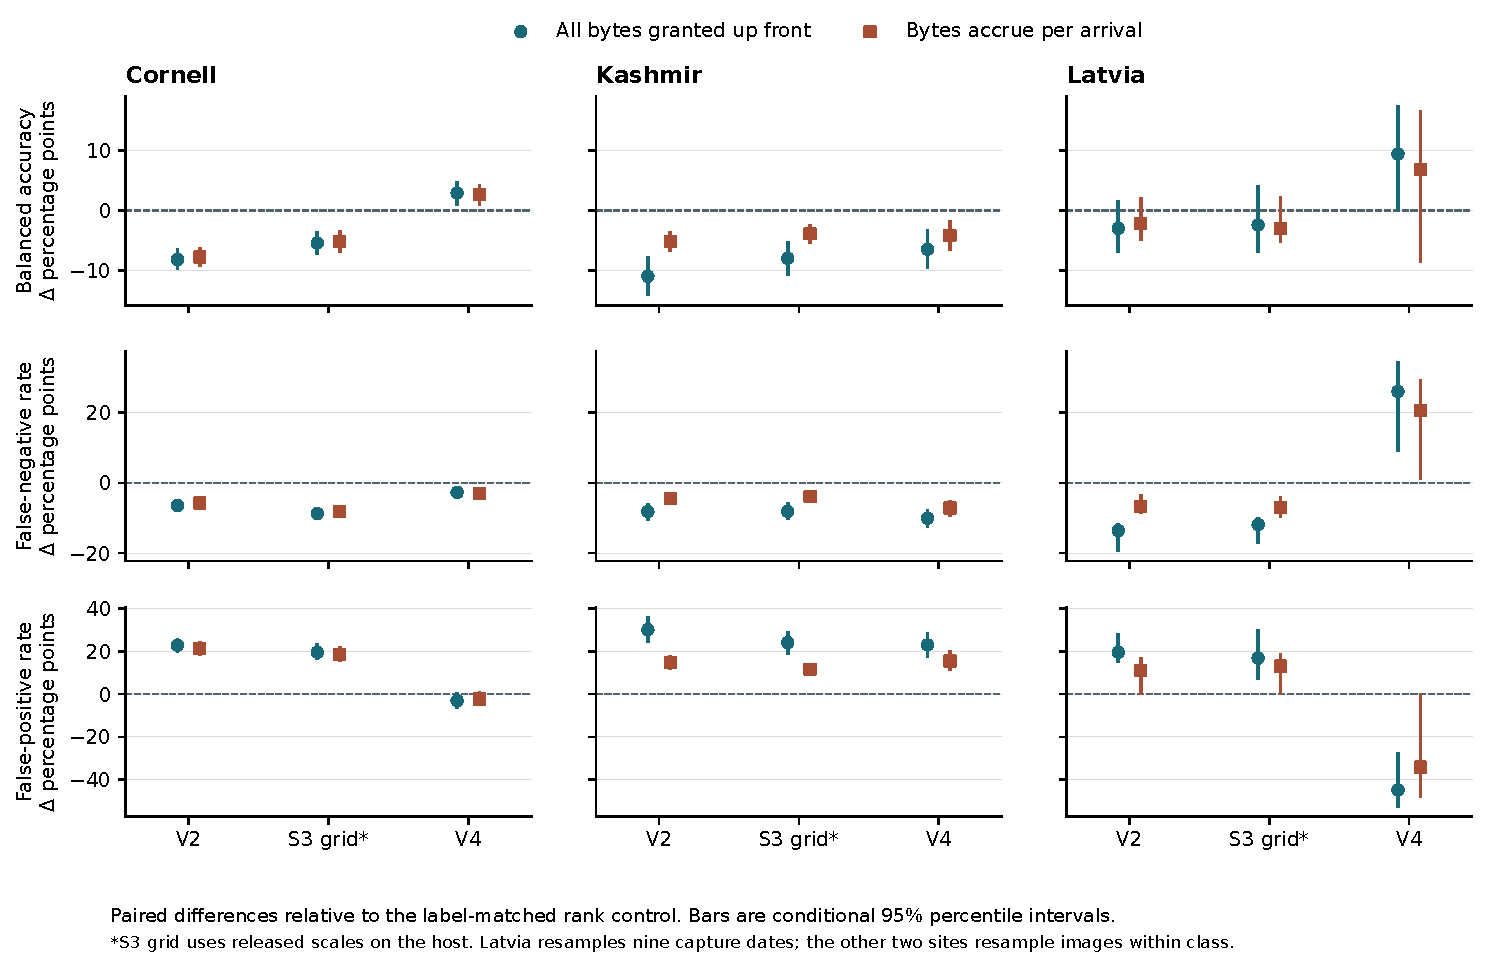
\includegraphics[width=.96\linewidth]{figures/purchase_effects.pdf}\end{center}
\note{Figure 2. Conditional paired effects across configurations. Equal actual label purchases and startup fees provide the reference. The zero-initial-credit comparison remains tied to each scheduled stream.}

\subt{Published routing differences can be smaller than precision shifts}
In a separate replay we keep the earlier Cornell 128-label training identities, the original three evaluation pools, orderings and byte allowances. This isolates quantization from the changed target-label policy. We reproduce all 1,540 original online comparisons at the level of decisions and queries and all 90 recorded core means in the historical batch table. Among 45 online method pairs, switching from FP32 to the host grid with the fitted head held fixed reverses 6 rankings on Cornell and 13 on Latvia. Re-fitting on grid features yields 0 and 10 reversals, respectively. All Kashmir methods fall back under this particular historical allowance.

In Cornell, continued balanced cross-entropy leads on FP32 at 85.66\% BA. OvA leads when serving uses grid features under a head fitted on FP32 (80.24\%). Continued balanced cross-entropy leads again after grid fitting (83.70\%). The quantization replay matches 59 of 60 archived forced board decisions but gives fixture codes $(56,-62)$ versus $(58,-59)$ in the release. This is sensitivity to the simulated numerical pipeline. Chip-level runtime, memory and energy require device measurements.
